\documentclass[9pt,a4paper]{article}

%%%%%%%%%%%%%%%%%%%%%%%%% packages %%%%%%%%%%%%%%%%%%%%%%%%

%\documentclass{aimsessay}
\usepackage[utf8]{inputenc}
\usepackage[english]{babel}

%Import the natbib package and sets a bibliography  and citation styles
\usepackage{natbib}
\usepackage{amsmath}
\usepackage{amssymb}
%\usepackage{natbib}
\usepackage{amsthm}
\usepackage{amsfonts}
\usepackage{graphicx}
%\usepackage{siunitx}
%\usepackage[utf8]{inputenc}
%\usepackage[english]{babel}
\usepackage[all]{xy}
\usepackage{float}
\usepackage{tikz}
\usepackage{verbatim}
\usepackage[left=2cm,right=2cm,top=2cm,bottom=2cm]{geometry}
\usepackage{hyperref}
\hypersetup{
	colorlinks=false,
	linkcolor=blue,
	filecolor=magenta,      
	urlcolor=cyan,
	pdftitle={Overleaf Example},
	pdfpagemode=FullScreen,
}
\usepackage{caption}
\usepackage{subcaption}
\usepackage{psfrag}

\usepackage{url} 
%\bibliographystyle{abbrvnat}
\usepackage{booktabs}  
\usepackage[T1]{fontenc}    % use 8-bit T1 fonts
%\usepackage[nottoc]{tocbibind}

\usepackage{url} 

\newcommand{\donna}[1]{{\color{red}{#1}}}   
\newcommand{\ignore}[1]{}

%%%%%%%%%%%%%%%%%%%%% students data %%%%%%%%%%%%%%%%%%%%%%%%
\newcommand{\student}{Brian KYANJO }
\newcommand{\course}{Fall-2021}
\newcommand{\assignment}{ Prof. Lejo Flores}


%%%%%%%%%%%%%%  Shortcut for usual set of numbers  %%%%%%%%%%%

\newcommand{\N}{\mathbb{N}}
\newcommand{\Z}{\mathbb{Z}}
\newcommand{\Q}{\mathbb{Q}}
\newcommand{\R}{\mathbb{R}}
\newcommand{\C}{\mathbb{C}}

%%%%%%%%%%%%%%%%%%%%%%%%%%%%%%%%%%%%%%%%%%%%%%%%%%%%%%%555
\begin{document}
	
	%%%%%%%%%%%%%%%%%%%%%%% title page %%%%%%%%%%%%%%%%%%%%%%%%%%
	\thispagestyle{empty}
	\begin{center}
		\textbf{Simulating Tropical Cyclone over the South-west Indian Ocean with
MPAS: Sensitivity to cloud microphysics schemes\\[0.5cm]
			Semester Project}
		\vspace{.2cm}
	\end{center}
	
	%%%%%%%%%%%%%%%%%%%%% assignment information %%%%%%%%%%%%%%%%
	
	\begin{center}
		\rule{17cm}{0.2cm}\\[0.3cm]
	\end{center}	
	
	\noindent	Name: \student \hfill Supervisor: \assignment\\[0.1cm]
	Semester: \course \hfill Date: \today\\
	\rule{17cm}{0.05cm}
	\vspace{.2cm}
	
	\section{Introduction}
	Tropical cyclones (TCs), one of the strongest atmospheric features, are known for massive destruction of properties and human lifes, because they are associated with strong winds, heavy rains, and storm surges \citep{TROPICAL}. Since the beginning of the 20th century, TCs have affected more than 629 million people and killed more than 1.33 million people in the tropics \citep{doocy2013human}. TCs, which usually form over warm tropical oceans ($\geq 26^{\circ}$C), are warm-core low-pressure systems with 100 - 1000 km diameter. Once established, TCs sustain their strength by absorbing warm moisture as they continue to enlarge and will last as long as the atmospheric and oceanic conditions remain favourable over the ocean. After making a landfall, TCs can last for seven days and cause severe damages as they move inland or along the coastline \citep{doocy2013human}. The TCs that form over the Southwest Indian Ocean (SWIO) are a threat to the neighbouring countries, but Madagascar, Mauritius and La Reunion experience the most devastating and destructive impacts of the TCs, followed by the extensive coastline and the borders of Zimbabwe and Mozambique \citep{Tropic}. For instance, in 2017, Tropical Cyclone Dineo (name of a tropical cyclone), which formed on 13th February and made a landfall over Mozambique on 15th February \citep{moses}. Dineo produced heavy rains (> 200mm  day-1) and damaging winds in Inhambane (southern province in Mozambique) and destroyed around 20000 homes, directly affected about  130,000 people, and killed seven people. Its widespread torrential rains and the associated storm surge produced massive floods that killed about 271 people and caused damages that exceeded \$ 200 million in Zimbabwe (USD 2017) \citep{Cyclone}. Although Dineo weakened on February 17th, its remnant low still triggered heavy rainfall with flooding in Botswana. The flooding destroyed 650 households and public infrastructures (e.g. bridges, hospitals, schools, and fields), leaving hundreds of people homeless and poor (especially the low-income earners) \citep{moses}. A month after the landfall, the impacts of Dineo landfall induced an outbreak of chlorella that infected 1,200 people and killed 2 people in Mozambique and Malawi \citep{Cyclone}. Despite the devastating impacts TCs over the region, from our best knowledge, there are still no reliable systems for providing early warning on TC occurrences over region. Hence, there is a need for more studies on how to improve simulation and prediction of TC characteristics over the SWIO. This will help reduce the devastating impacts of TCs in the region.
	
	%\section{Tropical cyclones (TCs)}
	
	
	\subsection{Problem Statement}
	Model for Prediction Across Scales (MPAS) cloud microphysics schemes: Weather Research Forecast (WRF)-Single-Moment-Microphysics Class 6 (WSM6) and Thompson, have a significant influence in the simulation of TC; however, according to past research, the capability of these two microphysics schemes in simulating TCs over the SWIO have not been tested yet. So comparing and analysing the influence of these microphysics schemes during simulations would help us to understand which scheme is best to use and under which available conditions. This will improve predictions of TCs over the basin and will reduce on the devastating damages caused by TCs ahead of time. 
	
	
	\subsection{Aim and objectives}
	This project aims to evaluate the capability of MPAS in simulating TC Dineo and examine the sensitivity of TC Dineo to two  prominent  cloud microphysics schemes: WSM6 and Thompson over the SWIO basin.
	
	The three specific objectives are:
	\begin{itemize}
		\item To describe the characteristics of TC Dineo.
		
		\item To evaluate how MPAS simulates TC Dineo over the SWIO basin.
		
		\item To compare the sensitivity of WSM6 and Thompson in the simulation of TC Dineo over the SWIO basin.
		
	\end{itemize}

		\section{Model Description}
		MPAS models use centroidal Voronic tessellations in their horizontal meshes, which provide a common software framework that gives an infrastructure for producing parallel execution, input, output, high-level driver program and other software infrastructure.  The supported important features of MPAS - Atmosphere (MPAS-A) include fully-compressible, non-hydrostatic dynamics, split-explicit Runge-Kunta time integration, Exact conservation of dry-air mass and scalar, Positive-definite and monotonic transport options, Generalised terrain-following hight coordinate. Unstructured variable-resolution (horizontal) mesh integrations for the sphere and Cartesian planes is also a supported vital feature of MPAS-A \citep{n.d.}. 
		
		Version 6.0 of MPA-A consists of parameterizations of physical processes that are taken from the WRF Model.  Explicitly Parameterizations of physical processes supported by MPAS-A include Radiation, Land-surface, Surface-layer, Boundary-layer, Convection, Cloud microphysics \citep{n.d.}. Table.~\ref{ps} shows the set of parameterizations of physical processes and their respective schemes. 
		

		
		
		MPAS-A consists of two  main components, i.e., the model and initialization, built as cores within the MPAS software framework. Both the model and initialization make use of software infrastructure and the same driver program but they are compiled as separate executables. The model component consists of physics and atmospheric dynamics. The initialisation component consists of components for creating initial conditions for the atmospheric and land-surface state and updating files for the sea-surface temperature (SST) and sea ice \citep{n.d.}. Figure.~\ref{components} shows model components within the MPAS framework. As shown in the Figure.~\ref{components} the init\textunderscore atmosphere (on the left) and atmosphere (on the right) are built as separate cores within the framework (MPAS superstructure). Both cores are symbolically linked to the MPAS common infrastructure (at the bottom).
		
		\begin{figure}[H]
			% Use "\centering" in floats (figure, table), but if you need to center
			% some text (why?) use "\begin{center}...\end{center}".
			\centering 
			% Figure environments same as 0.8 * \textwidth please
			% That does not necessarily mean the actual picture size,
			% it is a guideline for the environment which could contain
			% 2 or more pictures! Be consistent and follow the guidelines
			% provided in your sources.
			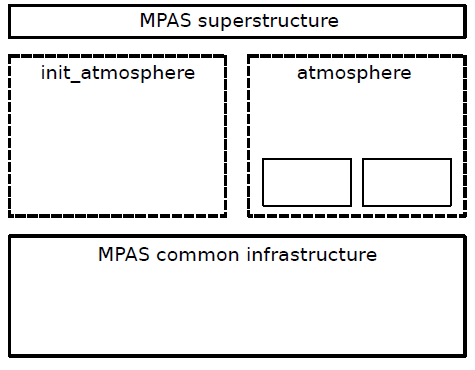
\includegraphics[width=0.8\textwidth]{images/componenets.png}
			\caption{The initialization and model components \citep{n.d.}}
			\label{components} 
			% if you move the label it breaks the reference numbering; 
			% always have it *after* the caption.
		\end{figure}
		
		\subsection{Dynamic core and physics of MPAS}
		The effect of physical processes on state variable evolution is modelled or represented using a generic term called Model physics. The effect of these processes is observed either when these processes like radiation, phases of changes of water species are not contained in the Navier-stokes equations  or when convective cells within coarse spatial resolution simulations are not resolved on the model mesh. Processes not to be resolved on the model mesh is caused by the failure of the structures to be represented on the mesh ($L<2\Delta x$), where L is the length of the grid and $\Delta x$ grid spacing. Inaccurate representation of present structures on the mesh in the dynamics below the effective resolution also causes physical processes not to be resolved on the model mesh. The physics operates on cell-centered variables. The radial-basis-functions reconstruction and cell-edge normal velocities are used to compute the global mesh and the components of cell-centered velocity \citep{ATMOS}. 
		
		The Physics in MPAS is divided into several parameterisations: microphysics, surface-layer, land-surface, short wave radiation, long wave radiation, boundary layer, convection, gravity wave drag by orography, and cloud fraction for radiation. Each parameterisation consists of different schemes for example, WSM6, Thompson and Kessler schemes are contained in microphysics, Noah is the only scheme in  land-surface whereas Tiedtke, New Tiedtke, Kain-Fritsch, and Grell-Freitas are schemes in convection parameterization etc. 
		
		
			\section{Data Needs}
			
		
		
		
		
			
				\section{Calibration}
				
				
					\section{Numerical Experiment Design}
					
	
	
	
		\bibliographystyle{abbrvnat}
	%\bibliographystyle{plain}
	\bibliography{references}
	
\end{document}

